%%%%%%%%%%%%%%%%%%%%%%%%%%%%%%%%%%%%%%%%%%%%%%%%%%%%%%%%%%%%%%%%%%%%%%%%%%%%%%%%
%% SUBSECTION: Metodologia badania
%%%%%%%%%%%%%%%%%%%%%%%%%%%%%%%%%%%%%%%%%%%%%%%%%%%%%%%%%%%%%%%%%%%%%%%%%%%%%%%%
\subsection{Metodologia badania}

Podstawą badania zużycia energii jest pomiar wartości pobieranego prądu przez zestaw uruchomieniowy
P-NUCLEO-WB55 w czasie. Posiadając dane wymienione dane, na podstawie oczywistych
zależności fizycznych wyznacza się parametry jak całkowita wykorzystana energia
podczas badania, przedstawiona w przystępnej postaci parametru mocy.

Pomiary wartości chwilowego poboru prądu oparto o moduł opisany w punkcie~\ref{device:plytka_pomiarowa}.
<<opis podłączenia + zdjęcie>>

\begin{figure}[!htb]
	\centering 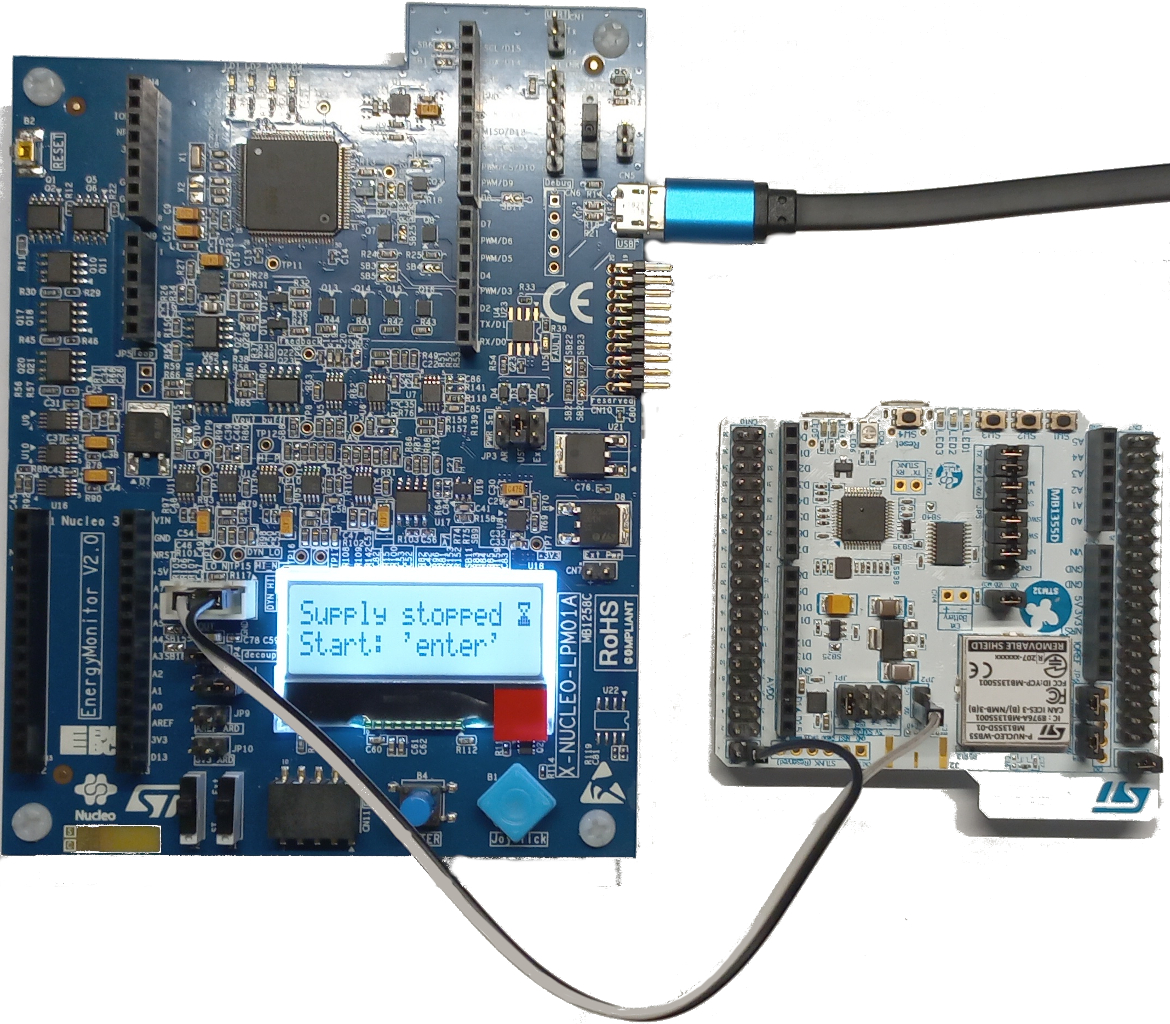
\includegraphics[width=0.618\linewidth]{power_measurement_unit_connected.png}
	\caption{Podłączony zestaw pomiarowy}
	\label{rys:connected_power_measurement_unit}
\end{figure}

Tak zebrane dane następnie przetworzono uzyskując wartości energii i średniej mocy
użytej przez układ. Wykorzystuje się w celu oczywistą zależność fizyczną zaprezentowaną
wzorem~\ref{energy_equation}\cite{skoro_marta_fizyka_1973}.

\begin{equation} \label{energy_equation}
E_{\text{całkowita}} = U \cdot \int_{t=0[s]}^{t=50[s]} \mathrm{d}i \: \mathrm{d} t
\end{equation}

\begin{equation} \label{power_equation}
P = \frac{E_{\text{całkowita}}}{t}
\end{equation}

gdzie:

\begin{description}
\item $E_{\text{całkowita}} [J]$ - wykorzystana energia podczas 50s sekundowej sesji rejestracji danych
\item $P [W]$ - moczużyta podczas 50s sekundowej sesji rejestracji danych
\item $U [V]$ - napięcie zasilania mikrokontrolera - 3.3V - stała
\item $\mathrm{d}i [A]$ - prąd w danej chwili
\item $\mathrm{d}t [s]$ - podstawa czasowa całkowania, 0.01s/interwał (100Hz) - stała 
\end{description}

Celem akwizycji danych wybrano dostarczane przez producenta oprogramowanie \textit{STM32CubeMonitor-Power}.
Pojedyncza sesja pomiarowa trwająca 100 sekund zapewnia niezbędne dane. Są one następnie
odpowiednio przetwarzane poprzez odcięcie wartości zebranych w ostatnich sekundach. Związane to było
ze sposobem działania mikrokontrolera, który po 60 sekundach przechodzi w stan zwiększonej
oszczędności energii. Stąd, by rozróżnić różne tryby pracy \gls{BLE}, zdecydowano o odcięciu
połowy okresu pomiarowego, zapewniając jednolite wartości względem trybów zużycia energii
w~50 sekundowym oknie.

Zebrane dane w postaci wartości chwilowych pobieranego przez mikrokontroler prądu względem czasu
przetworzono z użyciem metod numerycznych. W~celu wyliczenia łącznej wykorzystanej energii, a~tym samym
mocy, stosuje się zależność~\ref{energy_equation}. Uwzględniając fakt działania w domenie dyskretnej,
wykorzystano kompozytową metodę całkowania Simpsona~\cite{noauthor_scipyintegratesimpson_nodate}.
Podstawą dla całkowania są wartości zebrane w równoodległych odstępach. Dokonując akwizycji danych
dobrano częstotliwość próbkowania jako $100Hz$. Każda kolejna wartość charakteryzuje się więc
10 milisekundową różnicą w~podstawie czasu. Uwzględniając ten fakt, wyliczenie wartości
wykorzystanej energii jak i~mocy staje się trywialne.

\begin{figure}[!htb]
	\centering 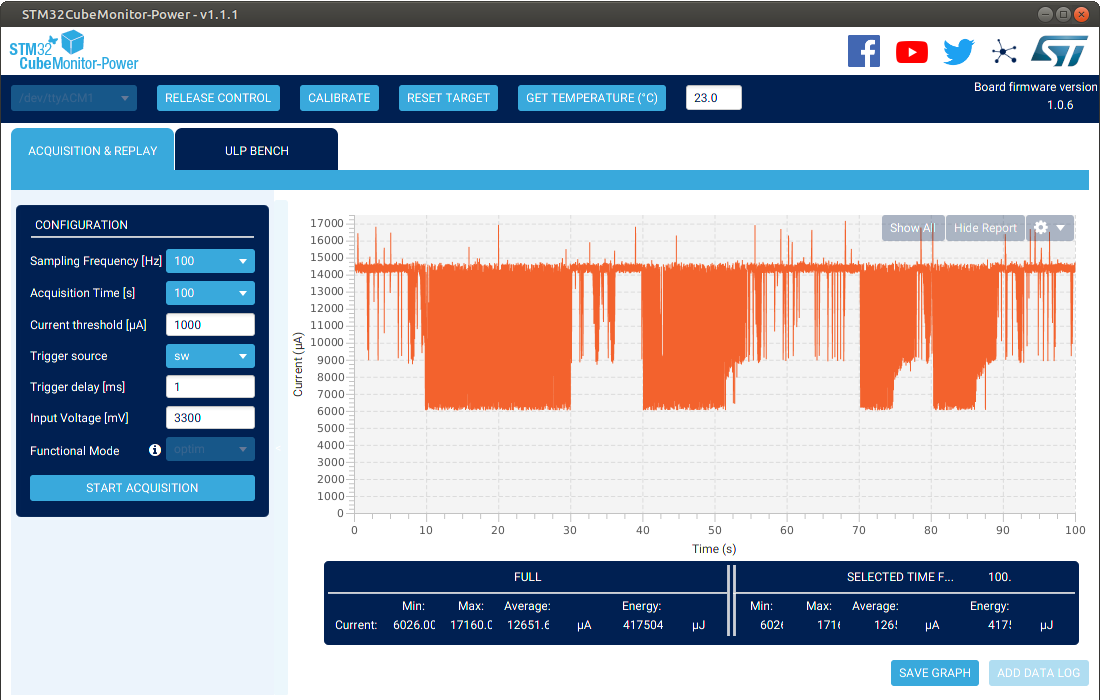
\includegraphics[width=0.99\linewidth]{stm32_power_monitor_sample.png}
	\caption{Przykładowa sesja pomiarowa dla BLE Mesh - sieć w trybie nasłuchującym}
	\label{rys:measurement_session_sample}
\end{figure}

%%%%%%%%%%%%%%%%%%%%%%%%%%%%%%%%%%%%%%%%%%%%%%%%%%%%%%%%%%%%%%%%%%%%%%%%%%%%%%%%
%% SUBSECTION: BT Low Energy - Usługa Heart Rate
%%%%%%%%%%%%%%%%%%%%%%%%%%%%%%%%%%%%%%%%%%%%%%%%%%%%%%%%%%%%%%%%%%%%%%%%%%%%%%%%
\subsection{BT Low Energy - Usługa Heart Rate}

\lipsum[1-3]
\begin{figure}[!htb]
	\centering 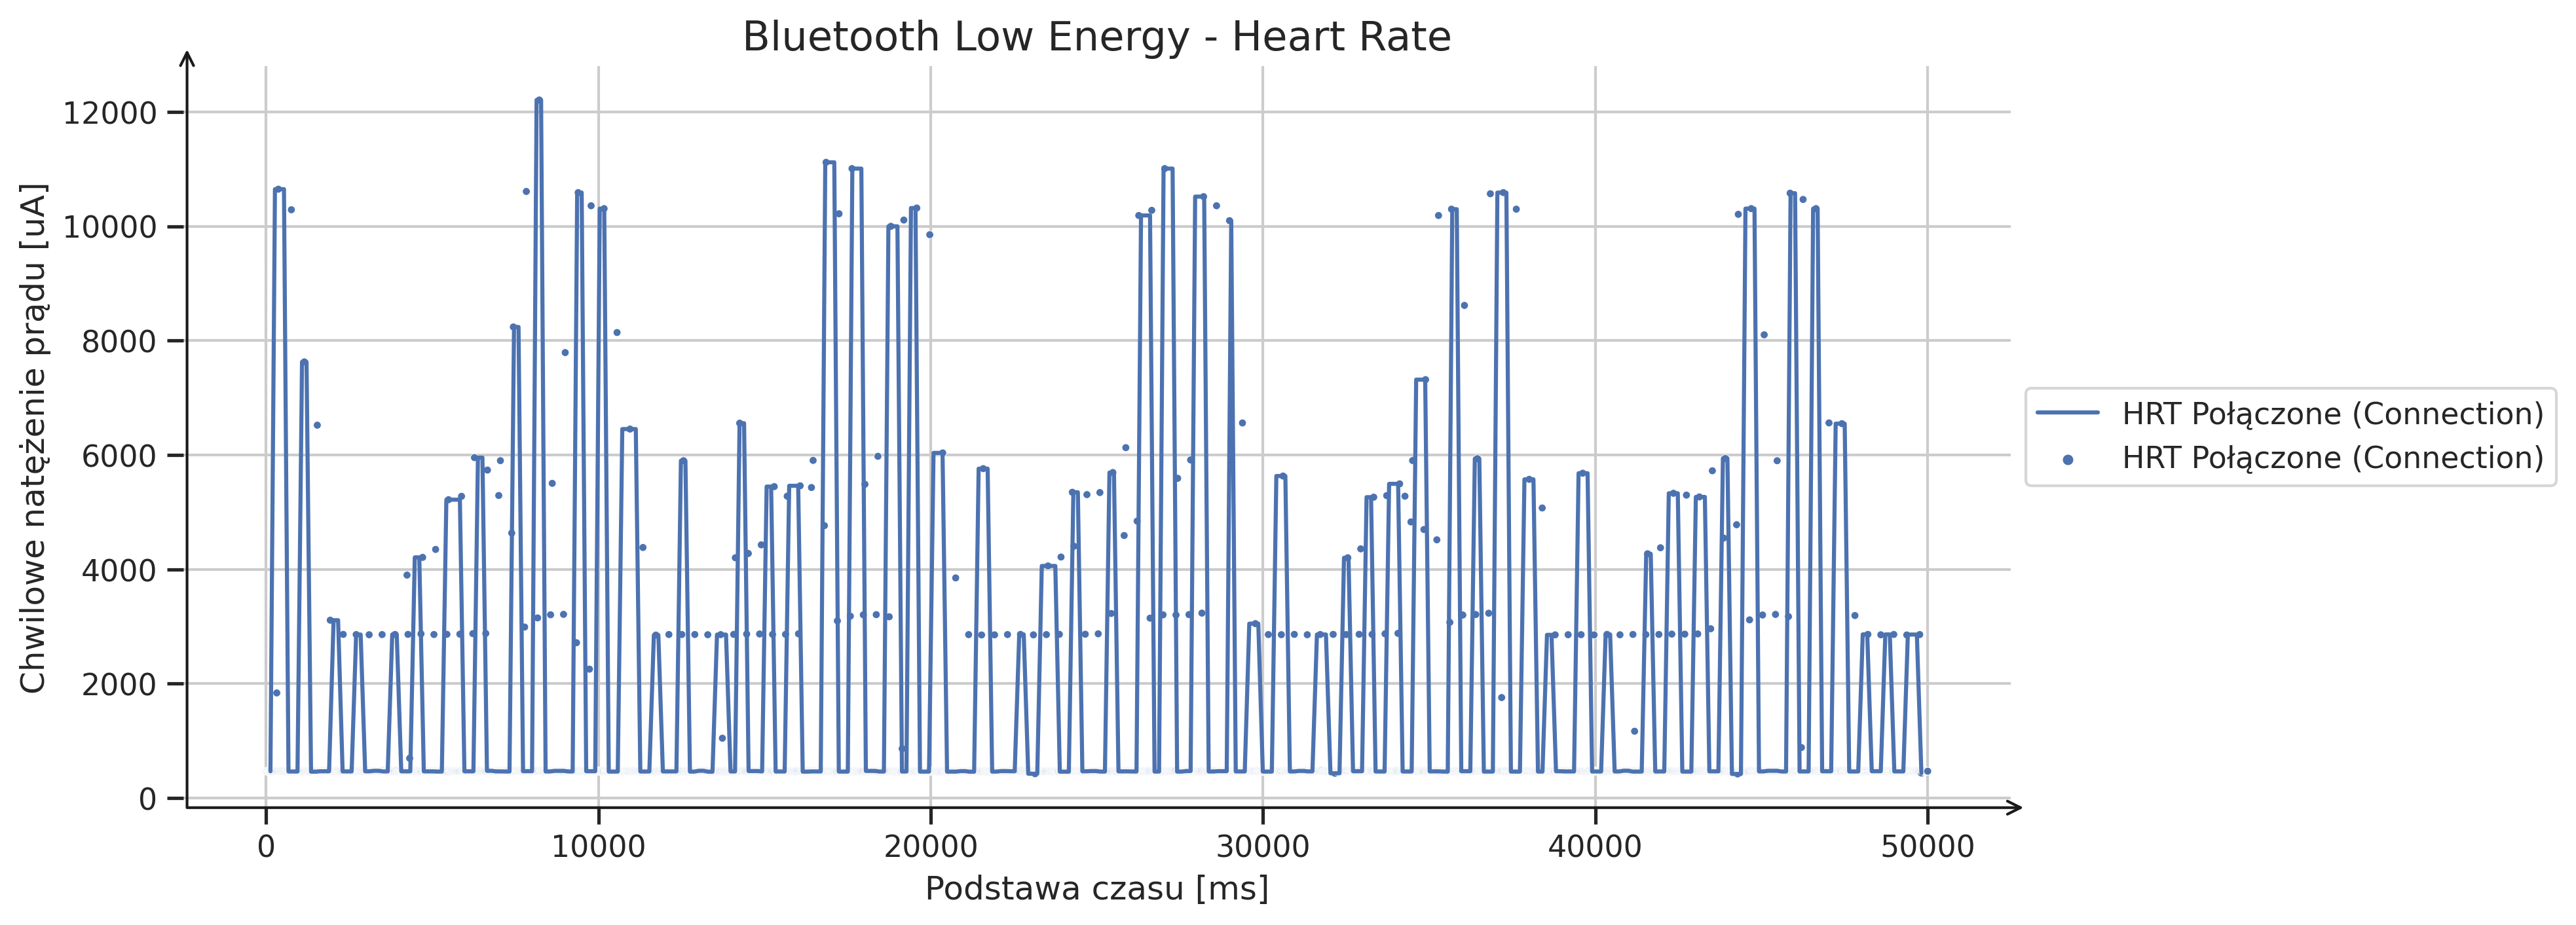
\includegraphics[width=0.99\linewidth]{power_ble_hr_connected_only_amps.png}
	\caption{Charakterystyka czasowa poboru prądu dla BLE i usługi Heart Rate - Usługa Połączona}
	\label{rys:power_ble_hr_connected_only_amps}
\end{figure}

\lipsum[1-3]
\begin{figure}[!htb]
	\centering 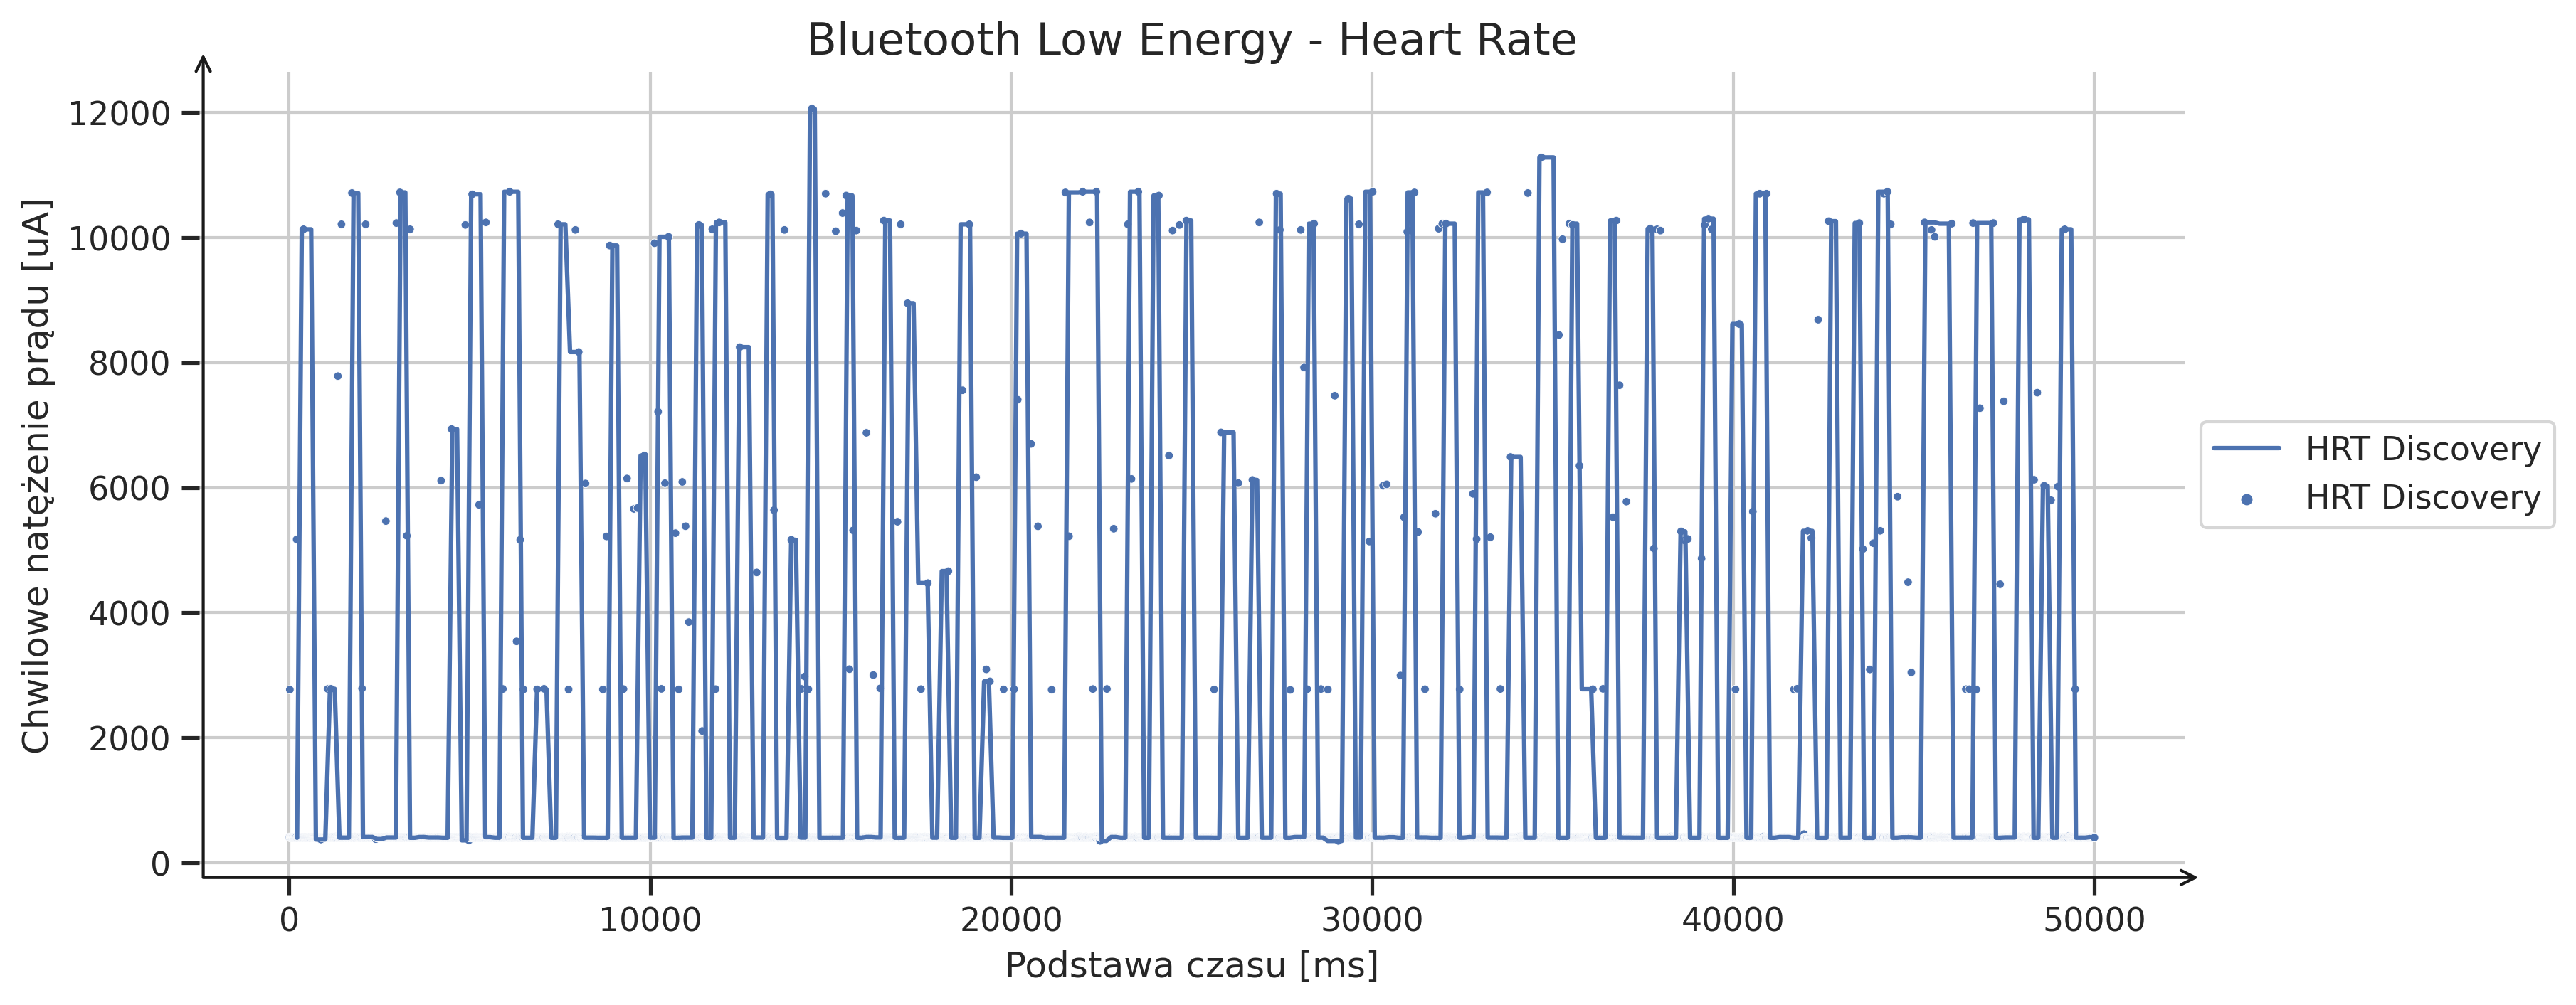
\includegraphics[width=0.99\linewidth]{power_ble_hr_discovery_only_amps.png}
	\caption{Charakterystyka czasowa poboru prądu dla BLE i usługi Heart Rate - Wyszukiwanie}
	\label{rys:power_ble_hr_discovery_only_amps}
\end{figure}

\lipsum[1-3]
\begin{figure}[!htb]
	\centering 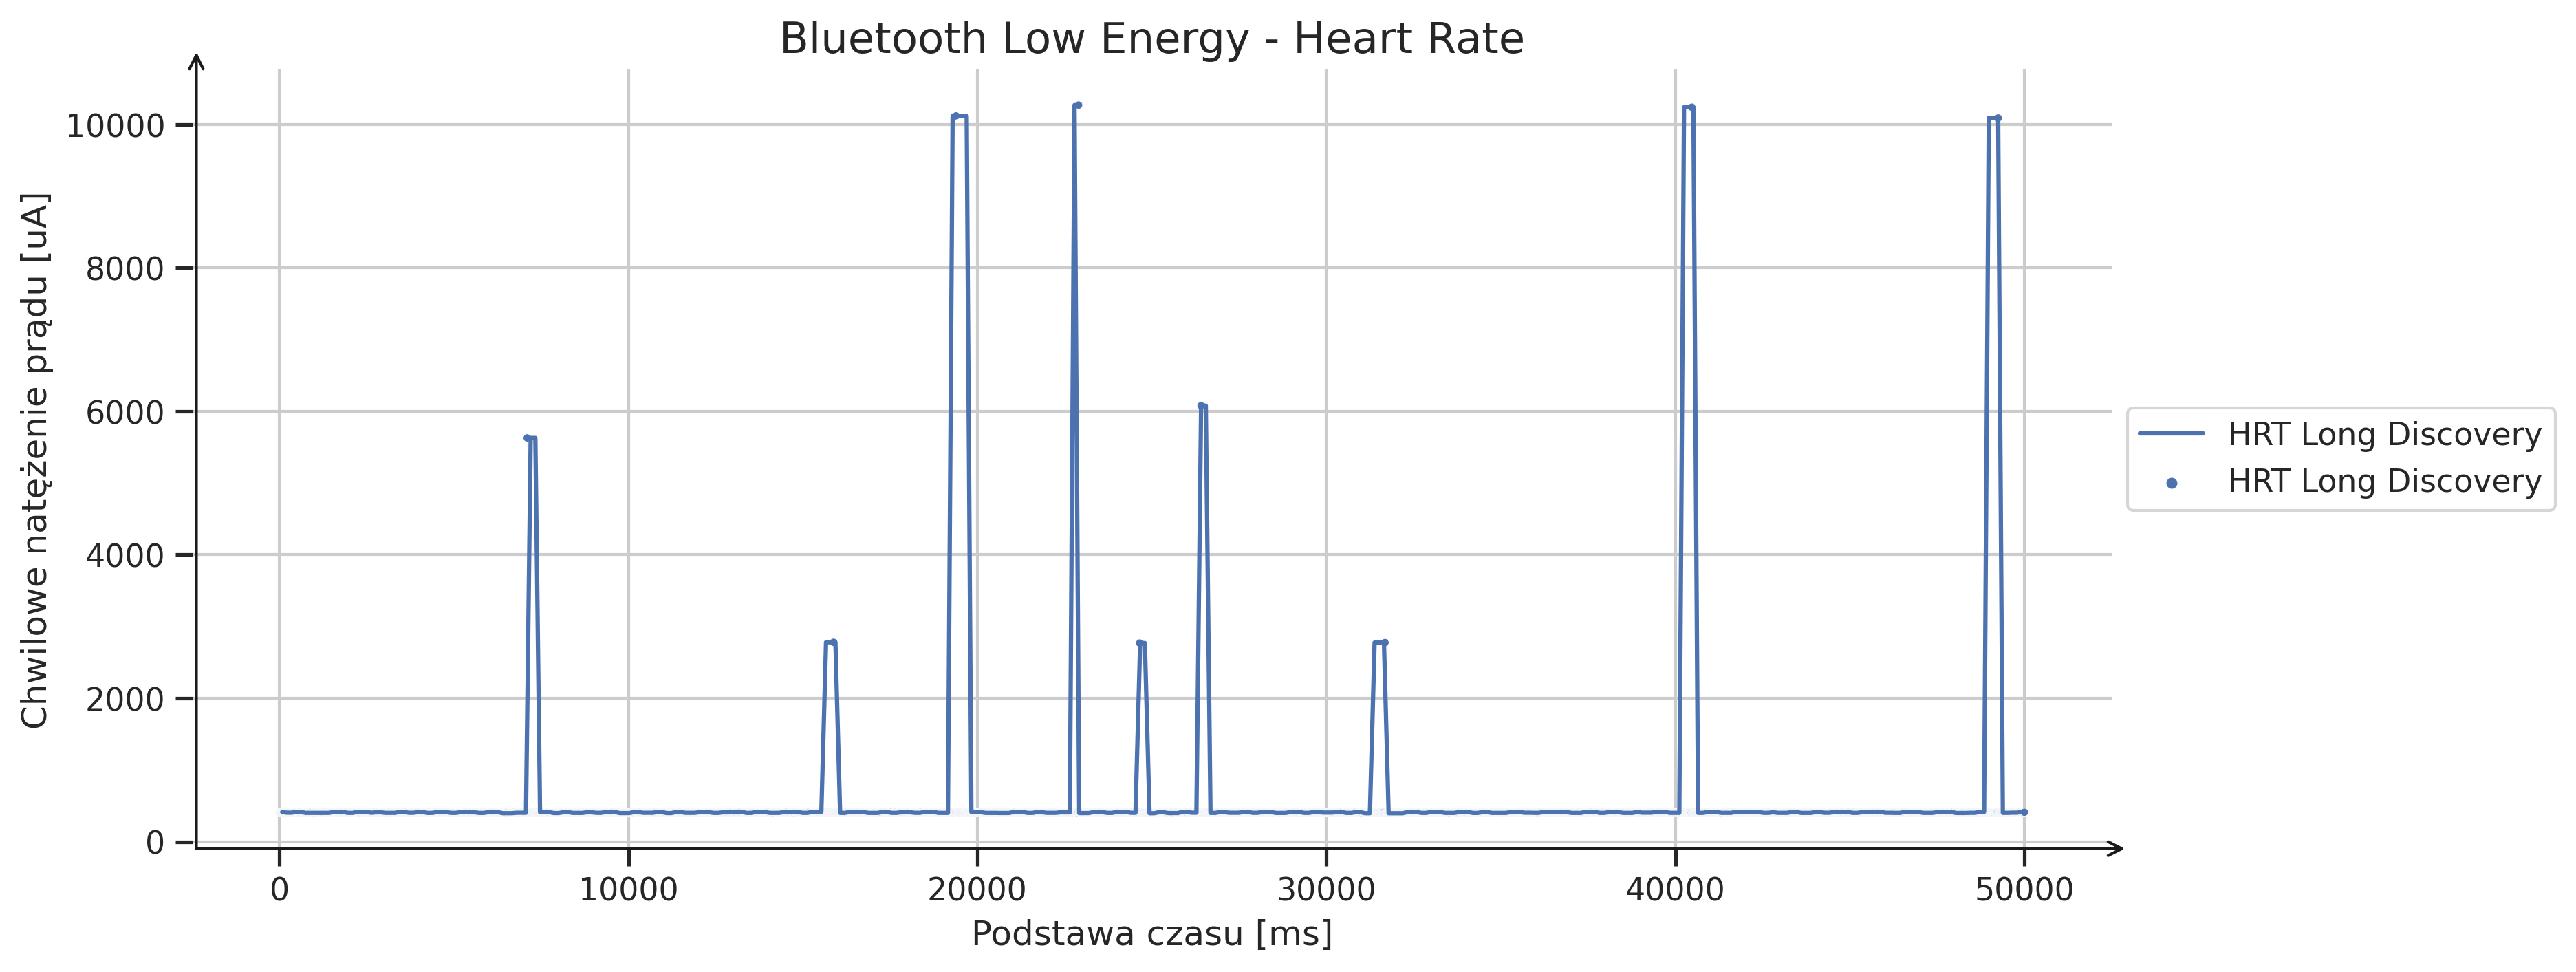
\includegraphics[width=0.99\linewidth]{power_ble_hr_long_connected_only_amps.png}
	\caption{Charakterystyka czasowa poboru prądu dla BLE i usługi Heart Rate - Wyszukiwanie, urządzenie w gotowości}
	\label{rys:power_ble_hr_long_connected_only_amps}
\end{figure}


\lipsum[1-2]
\begin{figure}[!htb]
	\centering 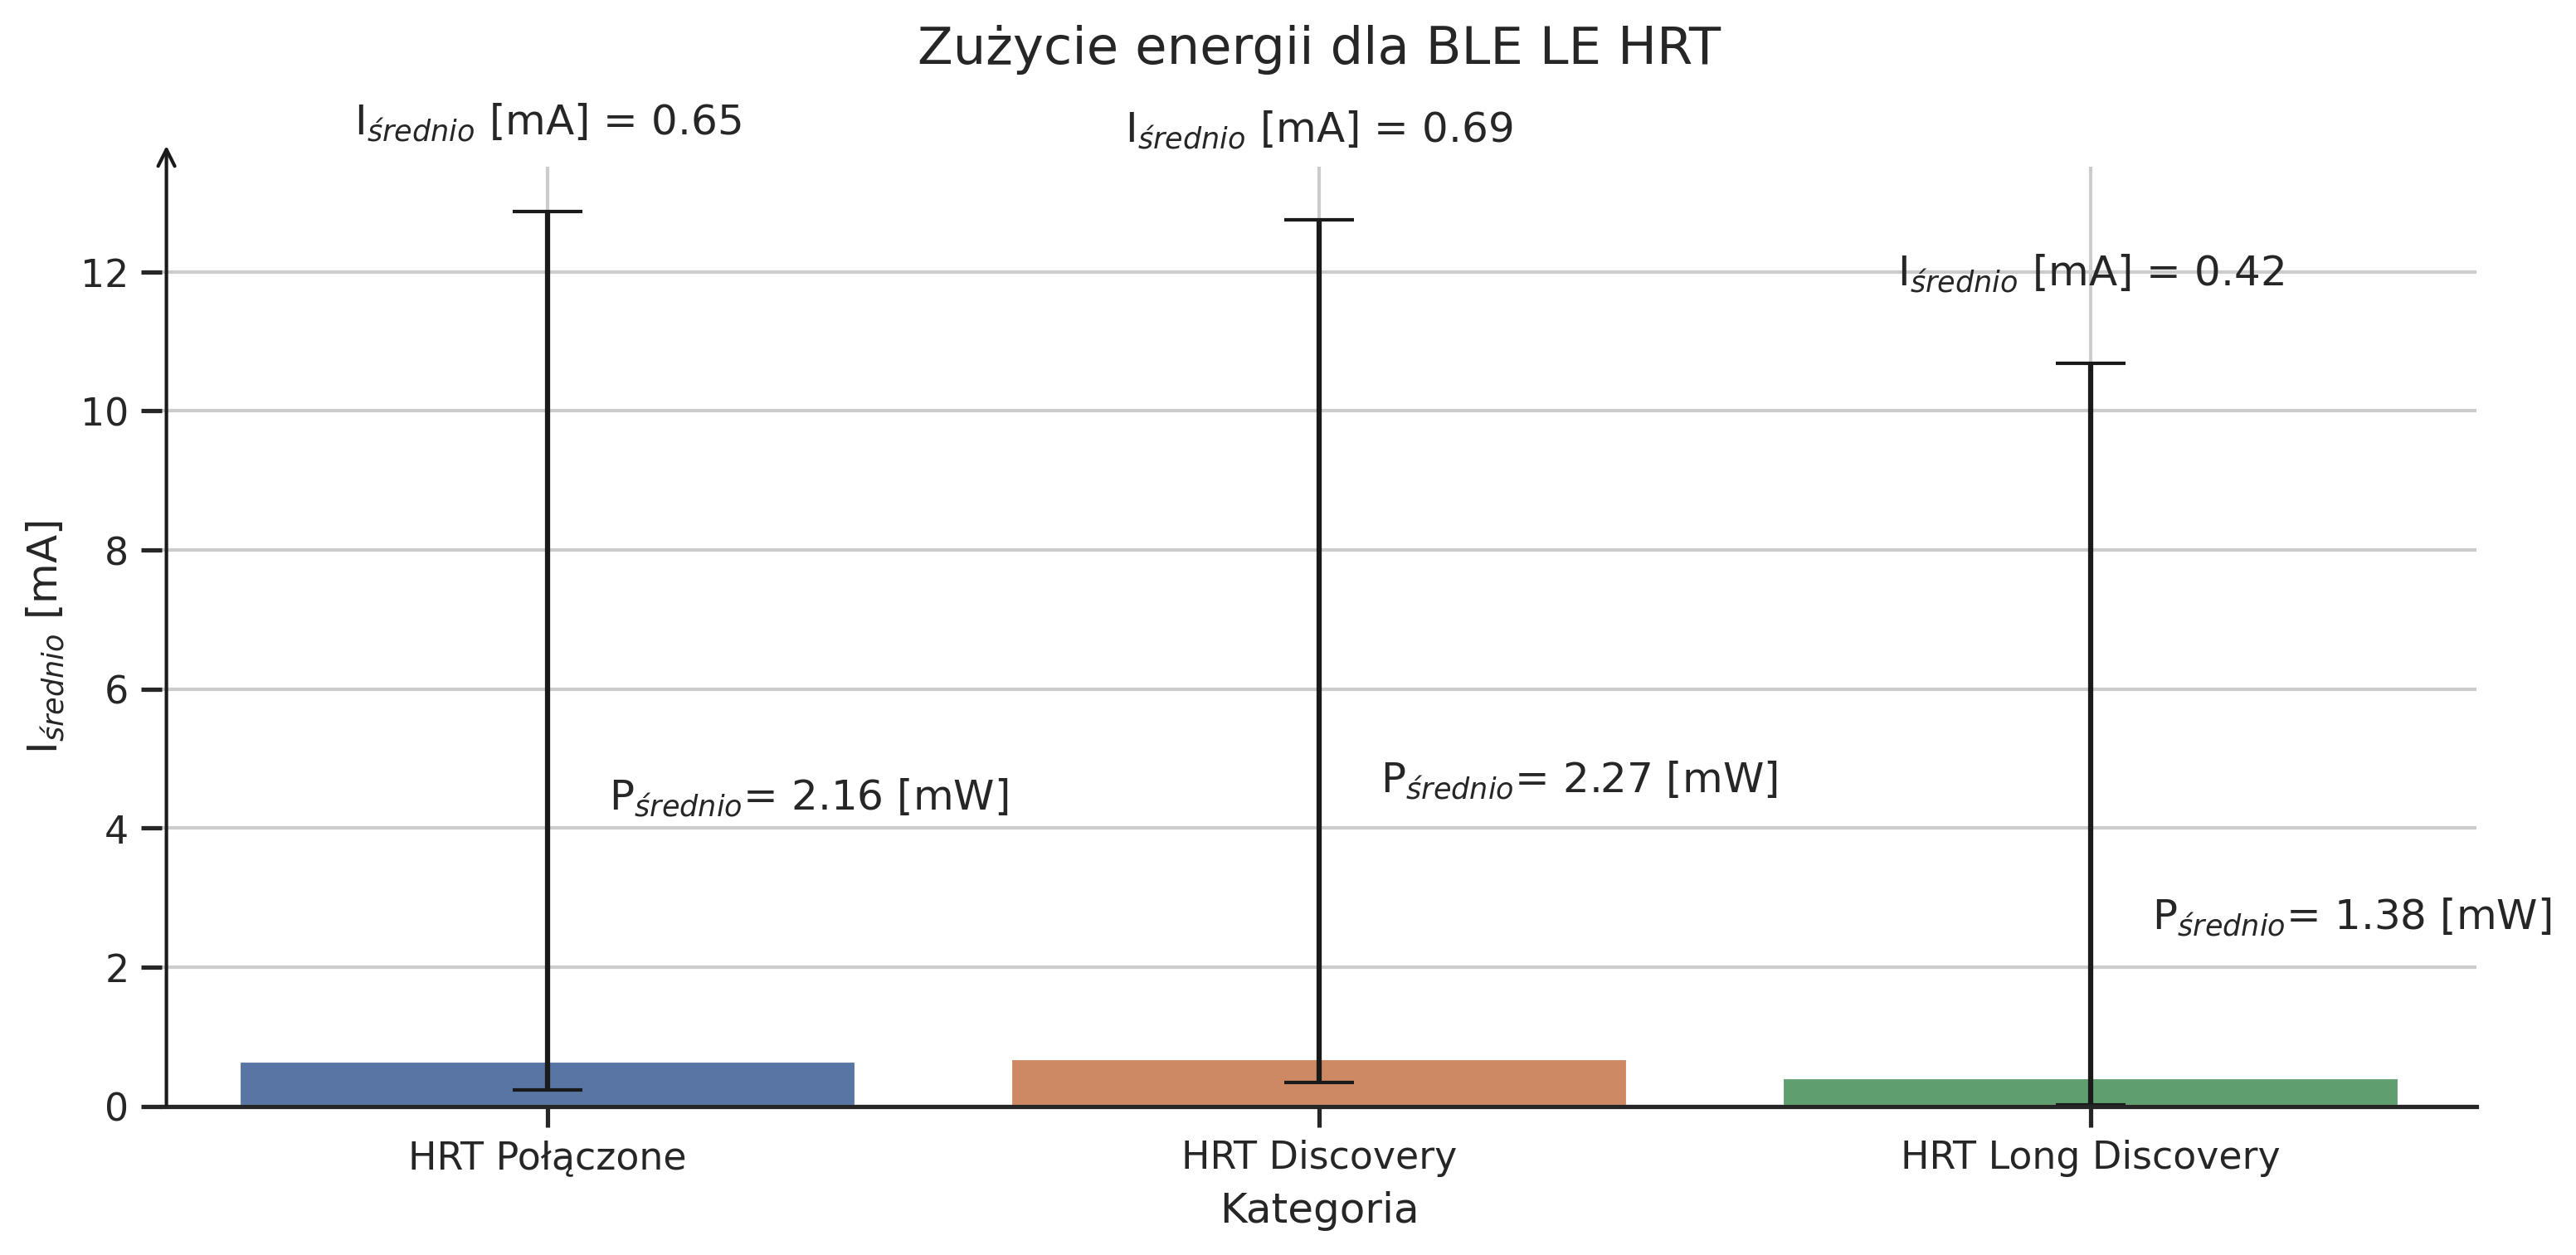
\includegraphics[width=0.99\linewidth]{power_ble_hr_amps_usage_juxtaposition.png}
	\caption{Zestawienie zużycia prądu dla usługi Heart Rate w zależności od trybu działania}
	\label{rys:power_ble_hr_amps_usage_juxtaposition}
\end{figure}
\lipsum[1-3]

%%%%%%%%%%%%%%%%%%%%%%%%%%%%%%%%%%%%%%%%%%%%%%%%%%%%%%%%%%%%%%%%%%%%%%%%%%%%%%%%
%% SUBSECTION: BLE Mesh - Model Generic OnOff
%%%%%%%%%%%%%%%%%%%%%%%%%%%%%%%%%%%%%%%%%%%%%%%%%%%%%%%%%%%%%%%%%%%%%%%%%%%%%%%%
\subsection{BLE Mesh - Model Generic OnOff}

Pomiary dla BLE Mesh uwzględniające dwa tryby działania: sieć w oczekująca na komunikaty oraz podczas działania aktywnego korzystania z Modelu Generic OnOff.

\begin{figure}[!htb]
	\centering 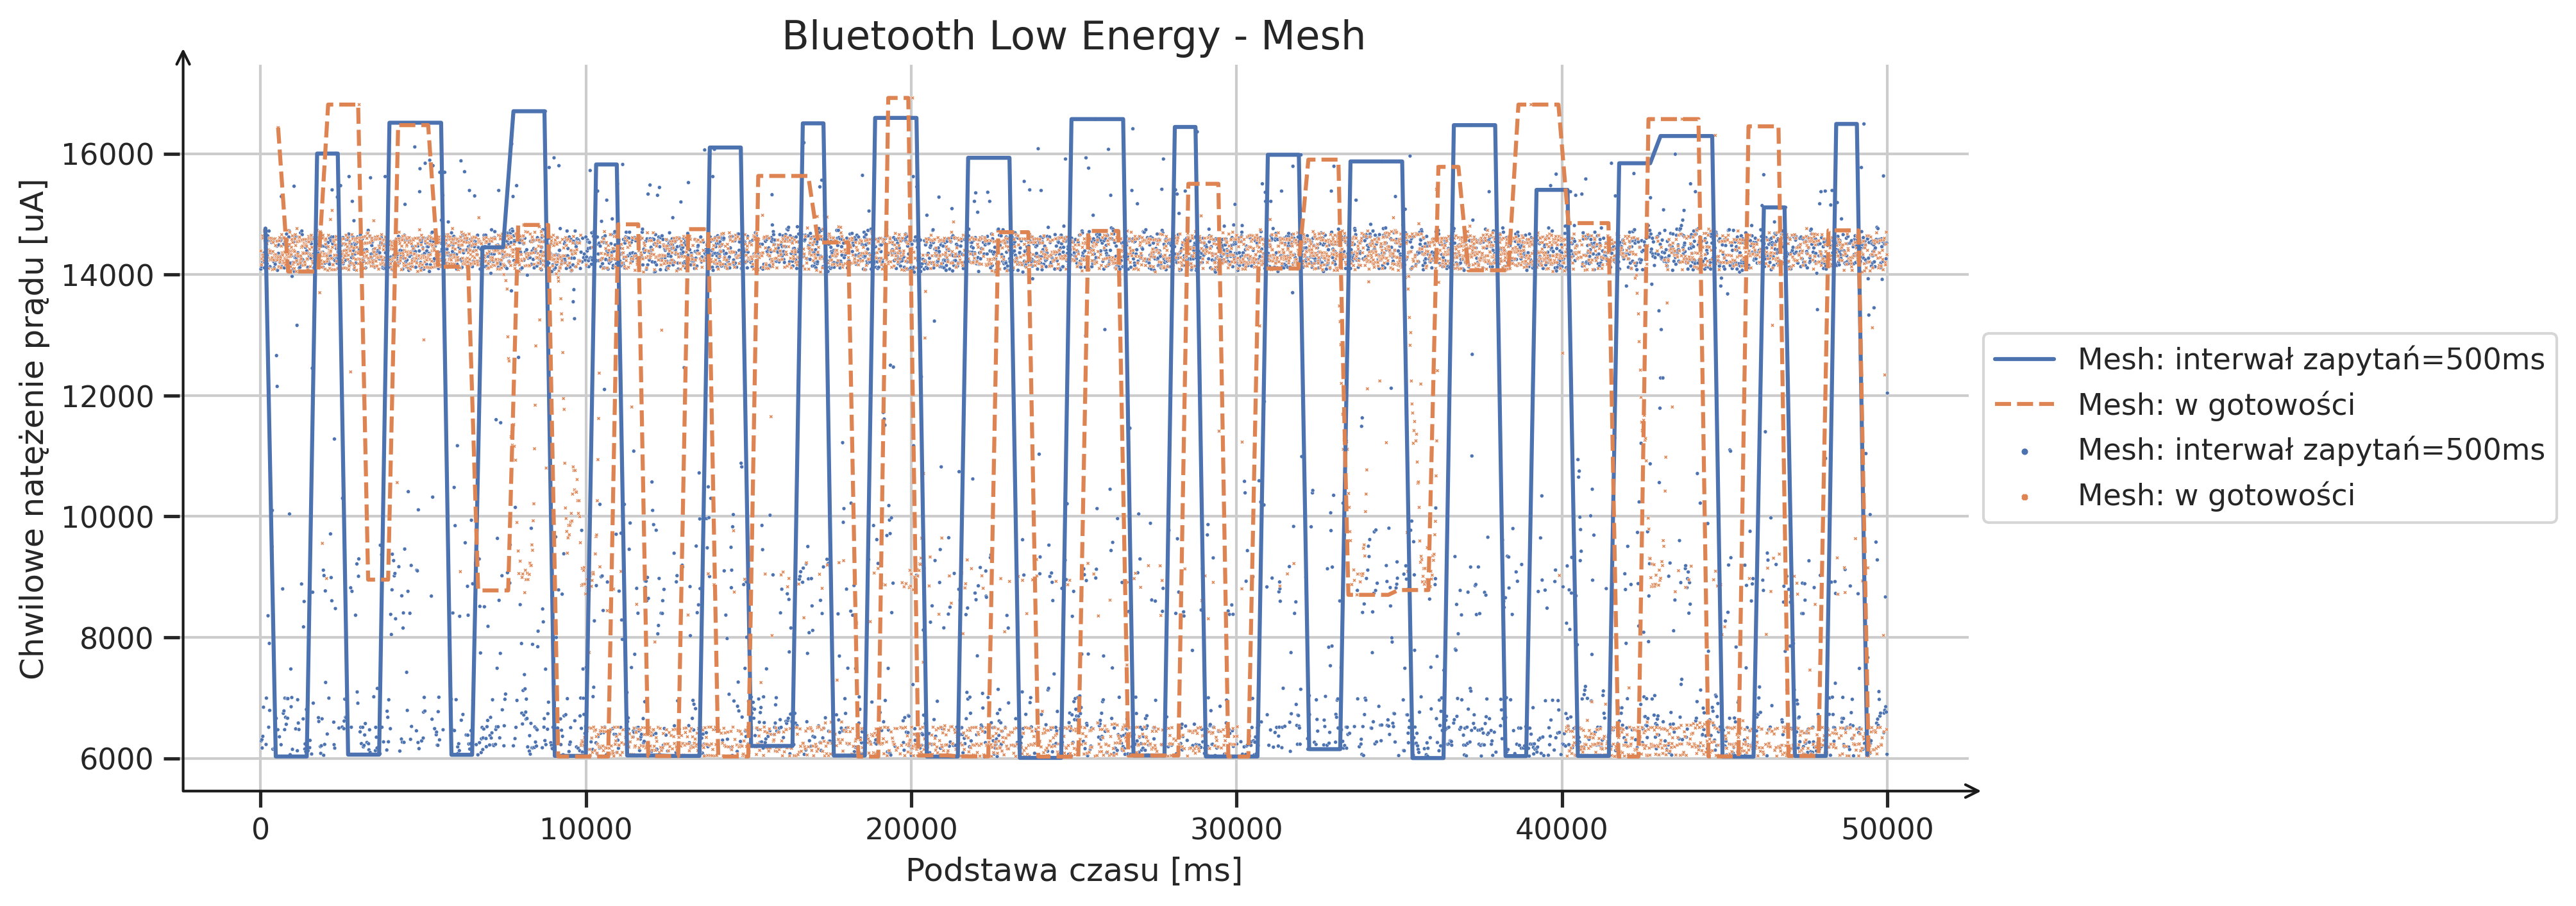
\includegraphics[width=0.99\linewidth]{power_ble_mesh_amps_no_led.png} 
	\caption{Charakterystyka czasowa poboru prądu dla BLE Mesh i modelu Generic OnOff}
	\label{rys:power_ble_mesh_amps}
\end{figure}

\lipsum[1-3]
\begin{figure}[!htb]
	\centering 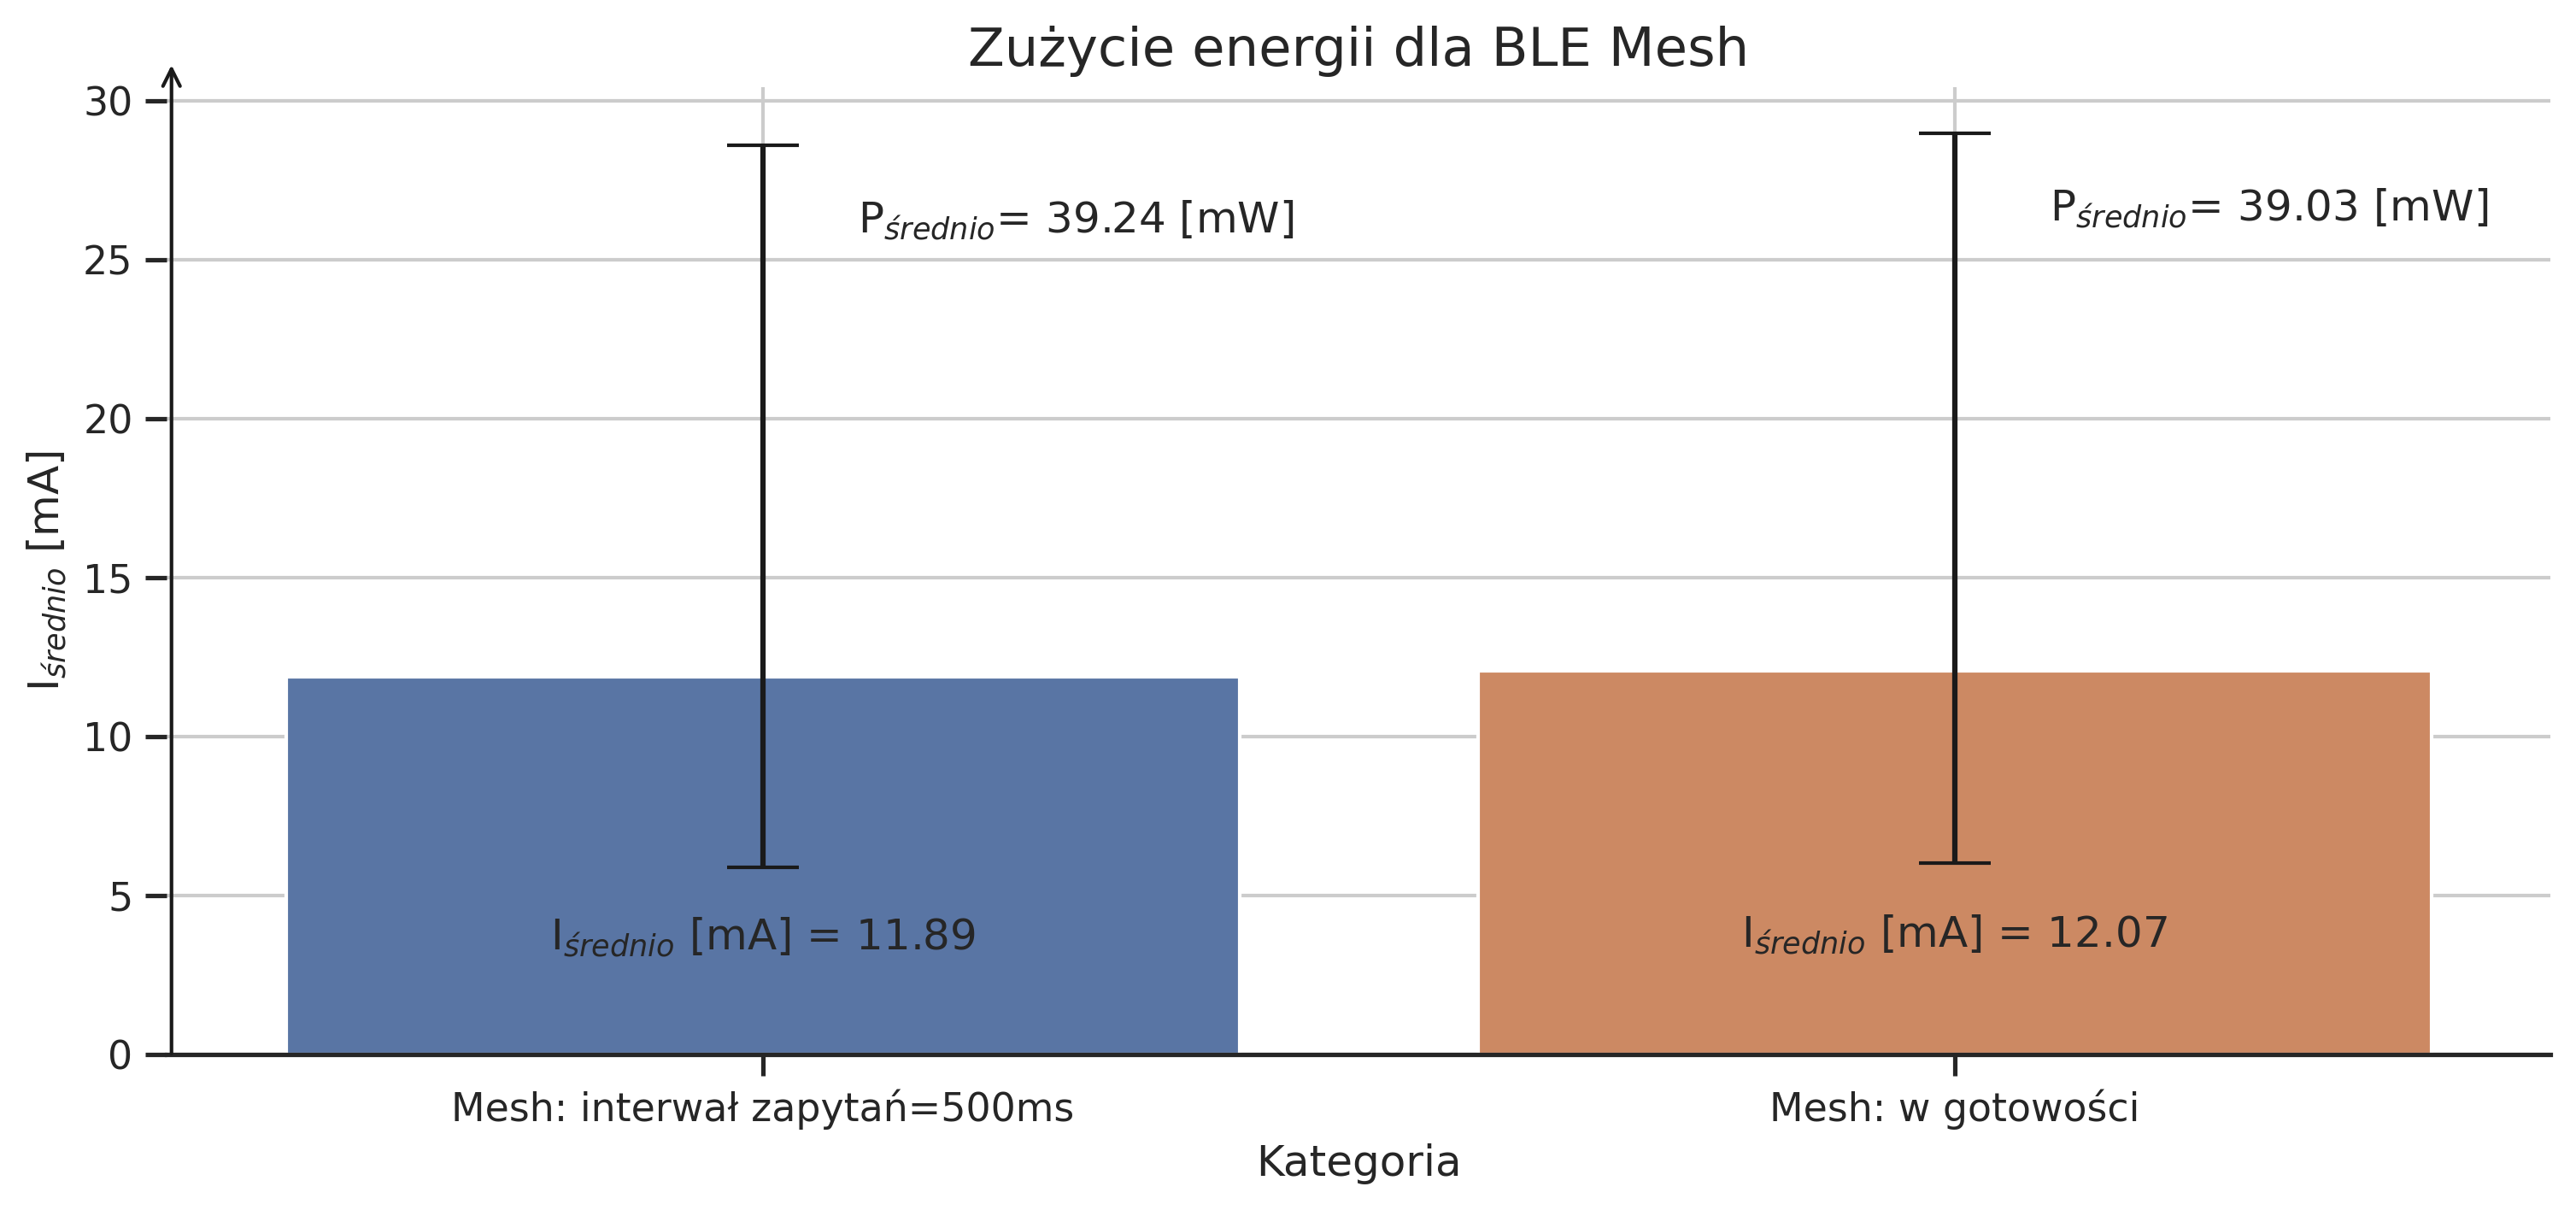
\includegraphics[width=0.99\linewidth]{power_ble_mesh_amps_usage_juxtaposition_no_led.png} 
	\caption{Zestawienie zużycia prądu dla BLE Mesh w zależności od trybu działania}
	\label{rys:power_ble_mesh_amps_usage_juxtaposition}
\end{figure}

\lipsum[1-3]
\begin{figure}[!htb]
	\centering 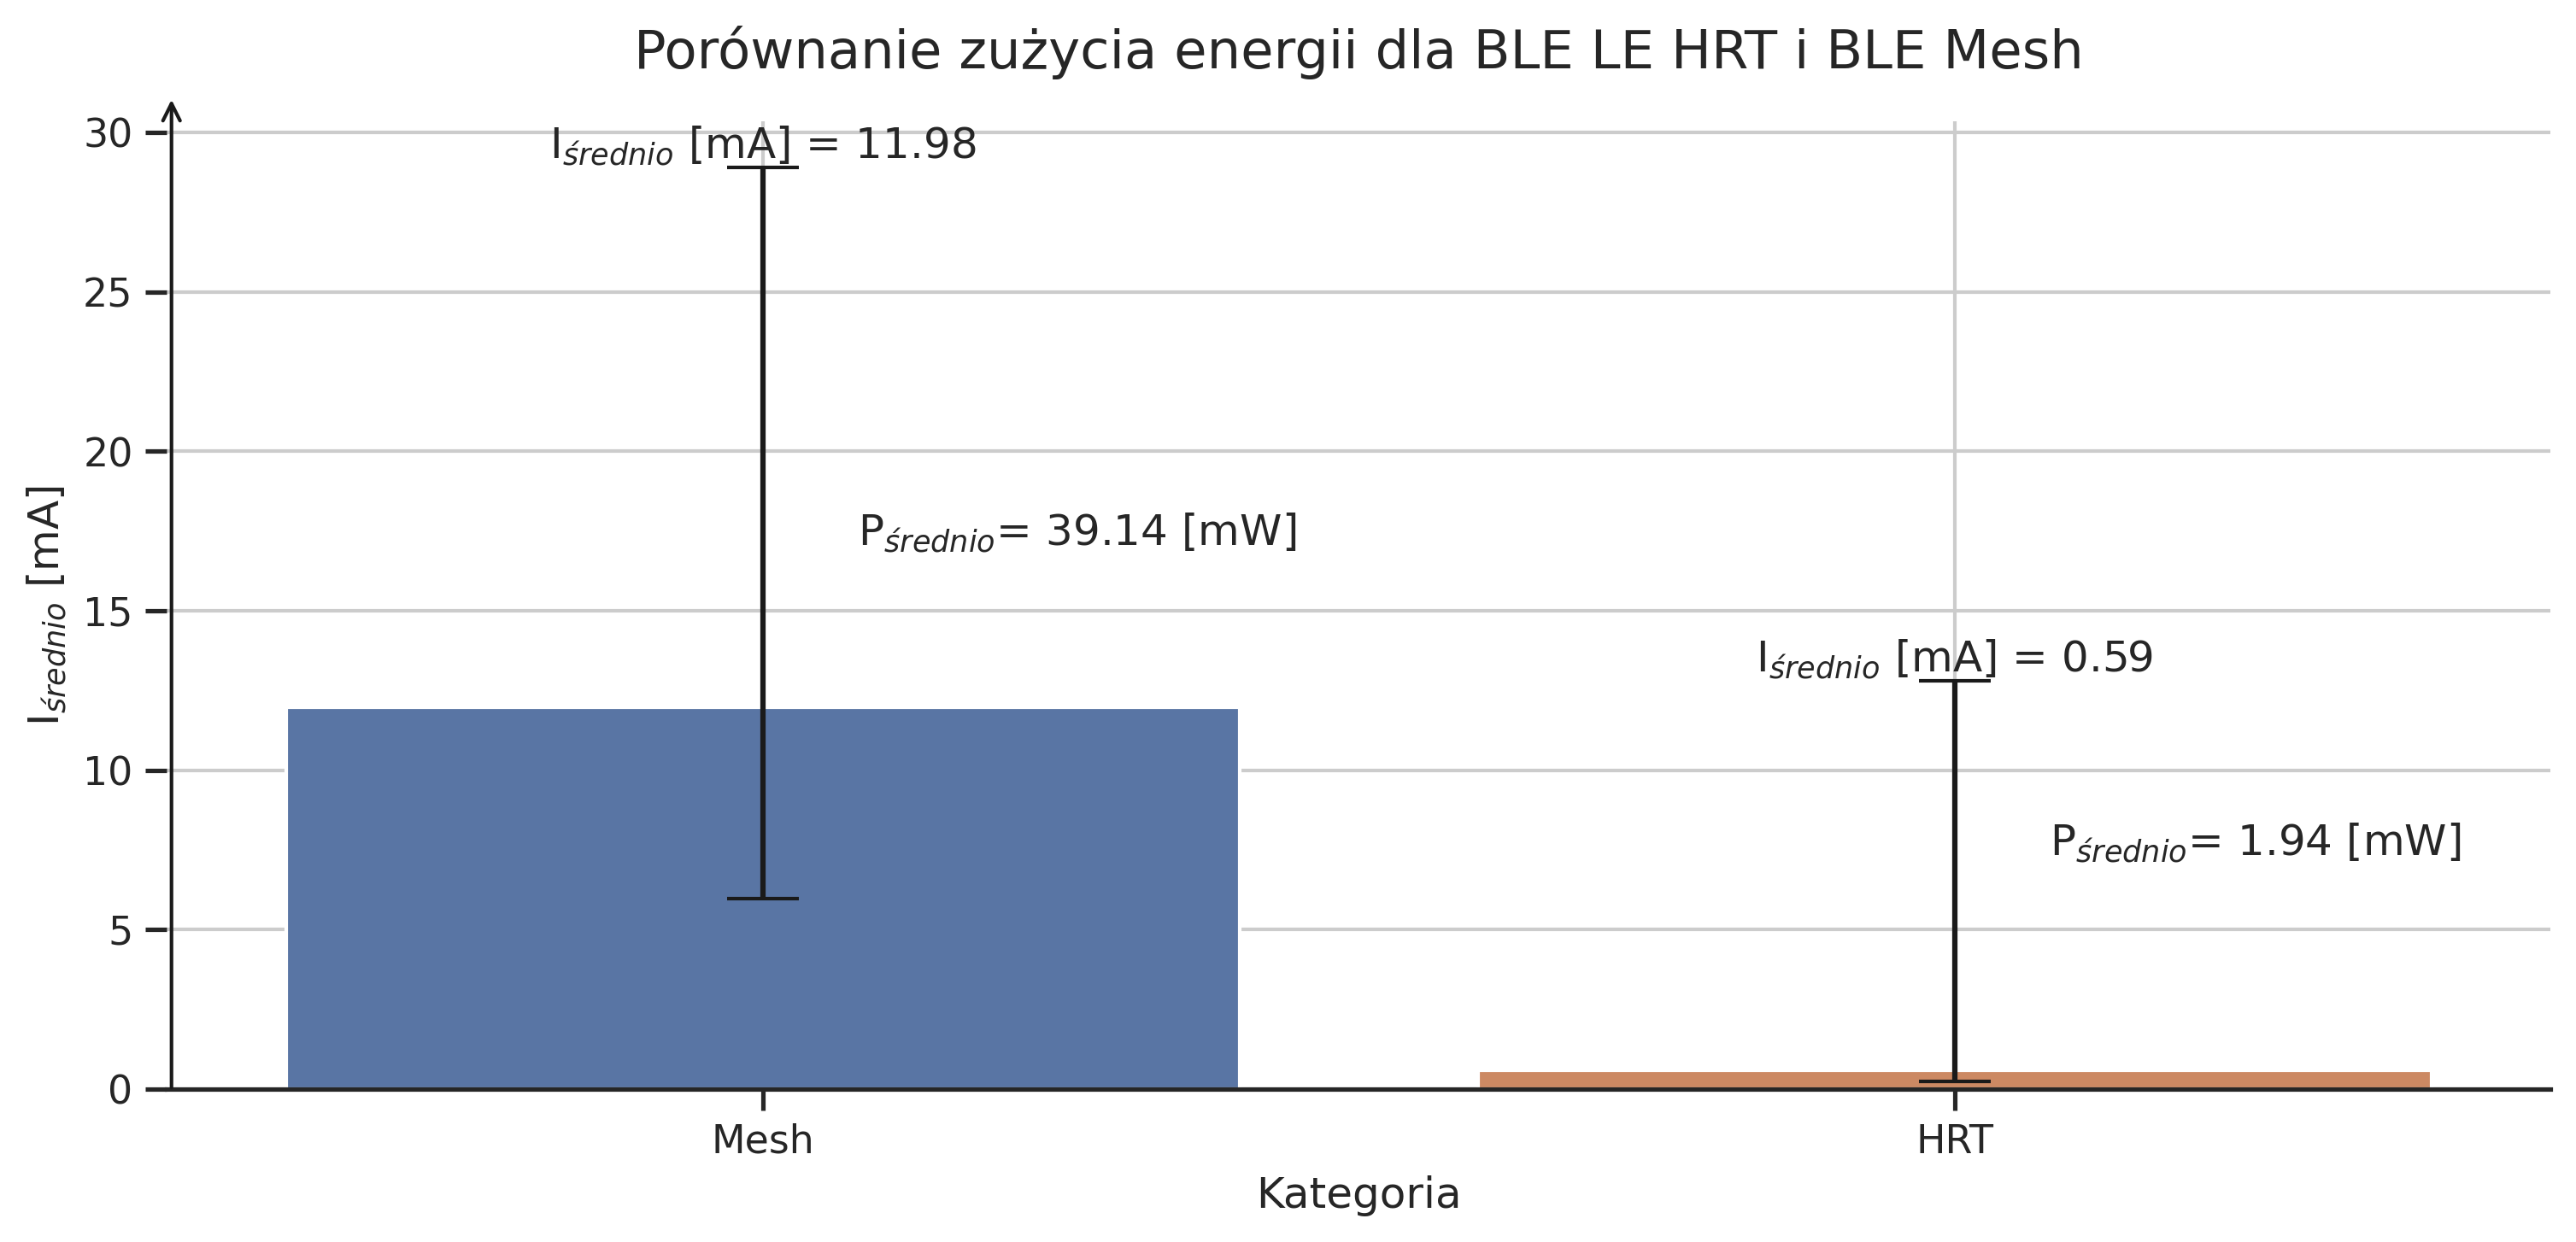
\includegraphics[width=0.99\linewidth]{power_ble_consumption_comparison_no_led.png} 
	\caption{Porównanie średniego zużycia energii pomiędzy BT Low Energy HRT i BLE Mesh}
	\label{rys:power_ble_consumption_comparison}
\end{figure}


